\que{Cвойства адиабаты Гюгонио.}
\paragraph{1.} Адиабата Гюгонио при любых фиксированных $ (p_1, V_1) $ невозрастает
        (см. предыдущий вопрос).

        \paragraph{2. Совершенный газ.} Подставим в адиабату выражение для
        внутренней энергии 
        \[
            \tilde{e}^0_2 - \tilde{e}^0_1 + \frac{p_2 V_2}{k - 1} -
            \frac{p_1V_1}{k-1} = \frac{1}{2} (p_1 + p_2) (V_1 - V_2).
        \]
        (См. предыдущий вопрос).


    \paragraph{3. Изменение энтропии вдоль адиабаты Гюгонио.} При непрерывном
    движении идеального газа имеет место соотношение $ \eta(p, \theta) \equiv
    \eta_0 $. Введём \emph{функцию Гюгонио} 
    \[
            H(p, V, p_1, V_1) := e(p, V) - e(p_1, V_1) + \frac{1}{2}(p_1 + p) (V
            - V_1).
    \]
    Зафиксируем $ p_1 $, $ V_1 $. Вычислим 
    \[
            dH = de + \frac{1}{2} (V - V_1)\, dp + \frac{1}{2} (p_1 + p)\, dV = 0.
    \]
   Этот дифференциал связывает точку на адиабате $ (p, V) $ с близкой $ (\tilde
   p, \tilde V)$, которая также лежит на адиабате и получена непрерывным
   движением (в отличие от точки $ (p_1, V_1) $). 

   Тогда используем формулу непрерывного движения $ de = \theta\, d\eta - p\, dV
   $ и получим  
   \begin{equation}
       \label{eq:deta}
       2\frac{dH}{dV} = 2\theta \frac{d\eta}{dV} + (V - V_1) \frac{dp}{dV} + (p_1 - p) = 0.
   \end{equation}
   Или, используя уравнение с тангенсом $ p - p_1 =  \tg\alpha \, (V - V_2) $
   (см. пред. вопрос), 
   \[
           2\theta \frac{d\eta}{dV} = (V_1 - V)^2 \frac{d}{dV} \tg \alpha.
   \]
   
\paragraph{4. Изменение энтропии вдоль адиабаты Гюгонио при малом скачке
удельного объёма.}
Рассмотрим уравнение \eqref{eq:deta}, где устремим $ (p, V) \to (p_1, V_1) $ и
получим $ d\eta (p(V), V) |_{V=V_1} = 0 $.

Используя ту же формулу, найдём  
\[
        2 \frac{d^2 H}{d V^2} = 2\theta \frac{d^2 \eta}{dV^2} + 2
        \frac{d\theta}{d\eta} \frac{d\eta}{dV} - (V_1 - V) \frac{d^2 p}{dV^2} +
        \frac{dp}{dV} - \frac{dp}{dV} = 0.
\]
Отсюда  
\[
        \theta \frac{d^2 \eta}{dV^2} = - \frac{d\theta}{dV} \frac{(V - 1 -
        V)}{\theta} \frac{dp}{dV} - \frac{d\theta}{dV} (p - p_1) + (V_1 - V)
        \frac{d^2 p}{dV^2}.
\]
Опять в силу непрерывности адиабаты $ V \to V_1 \Rightarrow p \to p_1 $ и $
\frac{d^2\eta}{dV^2}\big|_{V_1} = 0 $.

Аналогично вычислим третью производную 
\[
        2\frac{d^3 H}{dV^3} = 2 \frac{d\theta}{dV} \frac{d^2\eta}{dV^2} +
        2\theta \frac{d^3\eta}{dV^3} + 2 \frac{d^2\theta}{dV^2} \frac{d\eta}{dV}
        + 
        2 \frac{d\theta}{dV} \frac{d^2\eta}{dV^2} - (V_1 - V) \frac{d^3 p}{dV^3}
        + \frac{d^2 p}{dV^2} = 0.
\]
Тогда  
\[
    2\theta \frac{d^3\eta}{dV^3}\bigg|_{V_1} = - \frac{d^2 p}{dV^2}
    \bigg|_{V_1}.
\]

То есть при переходе из точки $ (p_1, V_1) $ в некоторую близкую ей точку $ (p,
V)$ с приращением $ \Delta V = V - V_1 $ вдоль адиабаты Гюгонио энтропия $
\eta $ в точке $ (p, V) $ меняется, но её изменение $ \delta \eta $ имеет третий
порядок малости по сравнению с $ \delta V $.

\paragraph{5. Взаимное расположение адиабат Гюгонио и Пуассона.} Адиабаты
Пуассона и Гюгонио для идеального газа имеют в точке $ (p_1, V_1) $ касание
второго порядка, причём левее этой точки адиабата Пуассона располагается ниже
адиабаты Гюгонио ($ \Delta\eta = \eta - \eta_1 > 0) $, а правее этой точки ---
наоборот, если (как для большинства газовых сред)
\[
    \frac{d^2 p}{dV^2}\bigg|_\eta > 0.
\]
В случае $ < 0 $ всё наоборот.
\begin{figure}[H]
    \centering
    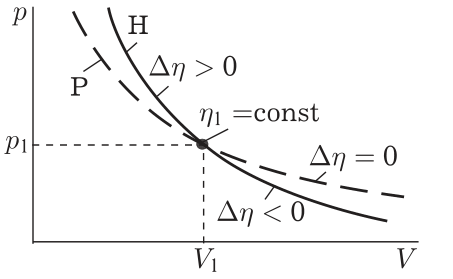
\includegraphics[width=0.4\textwidth]{img/puass+gug.png}
    \label{fig:puass-gug}
\end{figure}


